\documentclass[main.tex]{subfiles}

\begin{document}

\section{Aufgabe 2}
Von einer Zufallsvariablen $X$ wird vermutet, dass sie die nebenstehende Dichte $f$ besitzt mit $f(x) = 0$ für $x \neq [0; 3]$.
\begin{center}
	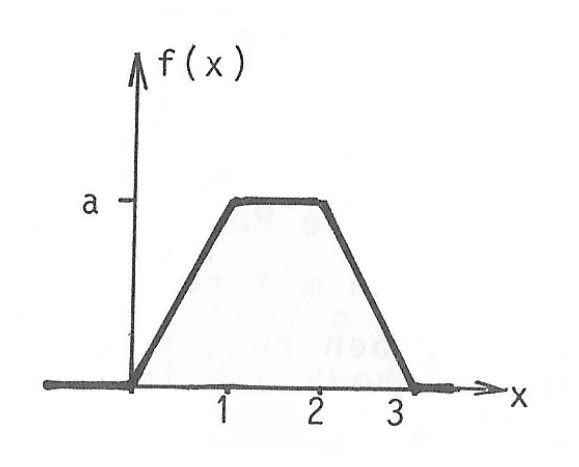
\includegraphics[scale=0.5]{Stochastik_III.4.10b_A02_Dichtefkt.jpg}
\end{center}
\begin{enumerate}
\item Bestimmen Sie die Konstante $a$ so, dass $f$ eine Dichte ist.
\item Testen Sie die Vermutung mit folgender Stichprobe zum Niveau $\alpha = 0,05$:
\begin{center}
	\begin{tabular}{c|c}
		Klasse & abs. Häufigkeit \\ \hline
		$[0; 1]$ & $15$ \\
		$(1; 2]$ & $29$ \\
		$(2; 3]$ & $6$
	\end{tabular}
\end{center}
\end{enumerate}

\subsection{Lösung 2}
Damit die Funktion $f$ eine Dichtefunktion sein kann, muss $\int_{-\infty}^{\infty} f(x) \dx{x} = 1$ sein. Dies ist der Fall für $a = 0,5$.

Bei einer Stichprobe vom Umfang $n = 50$ würde man unter Annahme der Dichte erwarten, dass Klasse $A_1$ im Intervall $[0; 1]$ und Klasse $A_3$ im Intervall $(2; 3]$ jeweils $E_{1,3} = 12,5$ Elemente, sowie Klasse $A_2$ im Intervall $(1; 2]$ $E_{2}=25$ Elemente enthält.  

Wir berechnen die Chi-Quadrat-Teststatistik $D$:
$$\begin{aligned}
	D &= \sum_{i=1}^{d} \frac{(O_i - E_i)^2}{E_i} \\
	&= \frac{(15 - 12,5)^2}{12,5} + \frac{(29-25)^2}{25} + \frac{(6-12,5)^2}{12,5} \\
	&= 4,52
\end{aligned}$$

Diesen Wert vergleichen wir mit dem 0,95-Quantil der Chi-Quadrat-Verteilung für $d-1 = 2$ Freiheitsgrade $\chi_{2;\ 0,95} = 5,991$.\\

Da $D=4,52 < 5,991 = \chi_{2;\ 0,95}$ können wir die Nullhypothese nicht ablehnen.

\end{document}
